\documentclass[DIV=calc]{scrartcl}
\usepackage[utf8]{inputenc}
\usepackage[T1]{fontenc}
\usepackage[ngerman]{babel}
\usepackage{graphicx}

\usepackage{fixltx2e}
\usepackage{ellipsis}
\usepackage[tracking=true]{microtype}

\usepackage{lmodern}                        % Ersatz fuer Computer Modern-Schriften
\usepackage{hfoldsty}

\usepackage{fourier} 			% Schriftart
\usepackage[scaled=0.81]{helvet} 	% Schriftart

\usepackage{url}
\usepackage{tocloft} 			% Paket für Table of Contents

\usepackage{xcolor}
\definecolor{urlred}{HTML}{660000}

\usepackage{hyperref}
\hypersetup{
  colorlinks=true,	
  linkcolor=black,	% Farbe der internen Links (u.a. Table of Contents)
  urlcolor=black,	% Farbe der url-links
  citecolor=black} % Farbe der Literaturverzeichnis-Links

\usepackage{mdwlist} 	% Änderung der Zeilenabstände bei itemize und enumerate

\parindent 0pt 				% Absatzeinrücken verhindern
\parskip 12pt 				% Absätze durch Lücke trennen

\usepackage{titlesec}	% Abstand nach Überschriften neu definieren
\titlespacing{\subsection}{0ex}{3ex}{-1ex}
\titlespacing{\subsubsection}{0ex}{3ex}{-1ex}		

% \pagestyle{empty}
\setlength{\textheight}{22,8cm}
\usepackage{fancyhdr}
\pagestyle{fancy}
\cfoot{}
\lfoot{Zusammenkunft aller Physik-Fachschaften\\Konferenz der deutschsprachigen Mathematikfachschaften}
\rfoot{zapfev.de\\die-koma.org}
\renewcommand{\headrulewidth}{0pt}
\renewcommand{\footrulewidth}{0.1pt}

\hyphenation{}

\begin{document}
\begin{minipage}{120pt}
\vspace{-2cm}
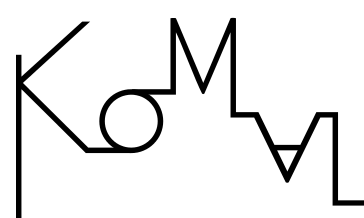
\includegraphics[width=100pt]{komaLogo.png}
\centering
\small Konferenz der deutschsprachigen Mathematikfachschaften
\end{minipage}
%\hspace{0.5\textwidth}
\hfill
\begin{minipage}{120pt}
\vspace{-2cm}

\includegraphics[width=80pt]{zapf_logo.pdf}
\centering
\small Zusammenkunft aller Physik-Fachschaften
\end{minipage}
\begin{center}
\huge{Positionspapier der Zusammenkunft aller Physik-Fachschaften und der Konferenz der deutschsprachigen Mathematikfachschaften} \\
\normalsize
\end{center}

%\vspace{1cm}
\section*{Rücktritt von Prüfungen}

Die 76. Konferenz der deutschsprachigen Mathematikfachschaften
und die Zusammenkunft aller Physik-Fachschaften
fordert, dass zum Rücktritt von Prüfungen an Hochschulen aus
gesundheitlichen Gründen ein ärztliches Gutachten zur
Prüfungsunfähigkeit ohne die Angabe von medizinischen Daten,
insbesondere Krankheit und Symptome, durch behandelnde Ärzt*innen
(Vertrauensärzt*innen der Hochschule oder Haus-/ Amtsärzt*innen)
gegenüber der Prüfungsbehörde als ausreichend gilt.

Dies soll verhindern, dass Studierende Diagnosen, Symptome und
vergleichbare medizinische Daten gegenüber der Hochschule offenlegen
müssen. Damit werden Datenschutzprobleme vermieden und die Prinzipien
der Datensparsamkeit und Datenvermeidung eingehalten.

Die 76. Konferenz der deutschsprachigen Mathematikfachschaften und
die Zusammenkunft aller Physik-Fachschaften würde
die Bereitstellung eines entsprechenden Formulars durch die Hochschule
begrüßen.

\vfill
\begin{flushright}
Verabschiedet durch die KoMa am 30.~Mai 2015 in Aachen\\
Verabschiedet durch die ZaPF am 31.~Mai 2015 in Aachen
\end{flushright}

\end{document}
